%% ----------------------------------------------------------------
%% 3_Chapter3.tex
%% ----------------------------------------------------------------
\chapter{REQUIREMENTS AND ANALYSIS}

This section will analyse the requirements of the proposed application and inform the design decisions that have been made.

\section{Use Cases}
    Use cases describe the various interactions between external actors and a given system as part of the Unified Modelling Language (UML). They are used in this section to define the interactions between users and the proposed application.

    \begin{figure}
        \center
        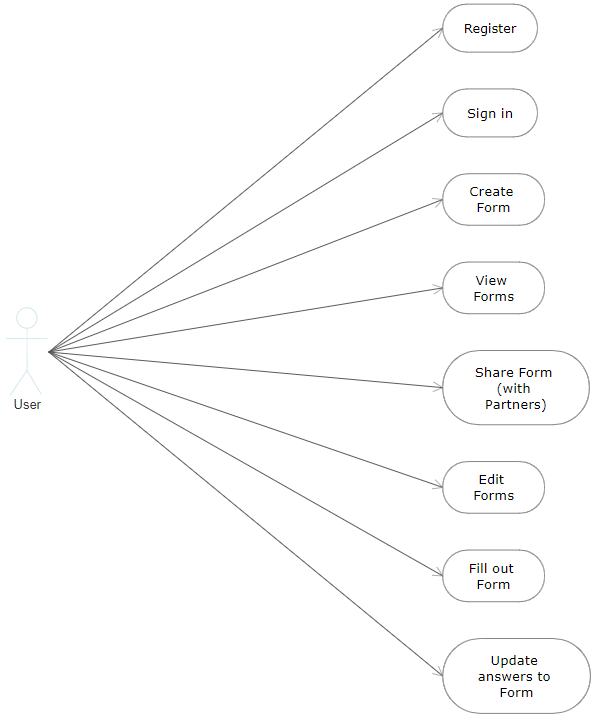
\includegraphics[height=100mm, width=150mm]{../figures/UseCaseUser}
        \caption{Use Case Diagram 1}
    \end{figure}

    \begin{figure}[h]
        \center
        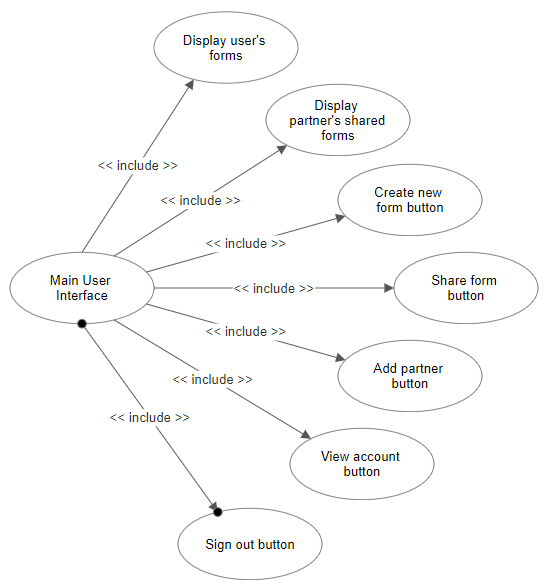
\includegraphics[width=150mm]{../figures/UseCaseInterface}
        \caption{Use Case Diagram 2}
    \end{figure}

    \clearpage

    \subsection{Use Case Description}

        The following table explains the major use cases for the application:\\

        \begin{table}[h]
            \centering
            \begin{tabular}{|c|c|}
                \hline
                Use Case & Description\\
                \hline
                \hline
                Display user's forms & \makecell{A list of forms created by the user will be displayed, with\\the form's name, owner and date of last modification.}\\
                \hline
                \makecell{Display partner's\\shared form} & \makecell{A list of forms shared with the user by a partner will be\\displayed, with the form's name, owner and date of\\last modification.}\\
                \hline
                \makecell{Create new\\form button} & Takes the user to a page where they can design a new form.\\
                \hline
                Share form button & \makecell{Allows the user to share forms they have created with partners.}\\
                \hline
                Add partner button & \makecell{Allows the user to search for other people's accounts on\\the application, and add them as partners. This should\\be done with other users that one would wish to share\\ forms with and/or receive forms from.}\\
                \hline
                View account button & \makecell{Allows the user to view their account information and edit\\it if necessary. Details such as name, email, company\\and the abilityto change the account's password.}\\
                \hline
                Sign out button & Allows the user to sign out from the application.\\
                \hline
            \end{tabular}
            \caption{Use Case Descriptions}
        \end{table}

\section{Functional Requirements}
    A functional requirement defines the intended behaviour of a component or part of a system. In the table below, the major functional requirements have been described:\\

    \begin{table}[h]
        \centering
        \begin{tabular}{|c|c|}
            \hline
            Requirement & Description\\
            \hline
            \hline
            Register & \makecell{New users will create an account before being allowed to use\\the application.}\\
            \hline
            Sign in & \makecell{Users will need to log in before they are able to\\access their account, create, share and complete forms.}\\
            \hline
            Create a form & \makecell{Users will be able to create a new form, which will be saved to\\their account.}\\
            \hline
            Share a form & \makecell{Users will be able to share a form that they have created with\\a partner.}\\
            \hline
            Add a partner & \makecell{Users will be able to view and edit their account information,\\including; name, email, company and password (not viewable).}\\
            \hline
            Sign out & Users will be able to sign out of the application.\\
            \hline
            Notifications & \makecell{Users will be notified of various changes, including their partners'\\answers to forms.}\\
            \hline
        \end{tabular}
        \caption{Functional Requirements}
    \end{table}

    \subsection{Functional Requirements Analysis}
        An importance level has been assigned to each of the functional requirements, in order to effectively plan the work to be done in order to create the minimum viable product. An additional table shows how the importance levels have been determined.\\

        \begin{table}[h]
            \centering
            \begin{tabular}{|c||c|c|c|c|c|}
                \hline
                Complexity/Time & Low & Medium & High\\
                \hline
                \hline
                Short & \cellcolor{green}0.0625 & \cellcolor{green}0.125 & \cellcolor{yellow}0.25\\
                \hline
                Medium & \cellcolor{green}0.125 & \cellcolor{yellow}0.25 & \cellcolor{red}0.5\\
                \hline
                Long & \cellcolor{yellow}0.25 & \cellcolor{red}0.5 & \cellcolor{red}0.75\\
                \hline
            \end{tabular}
            \caption{Importance Levels}
        \end{table}

        \begin{table}[h]
            \centering
            \begin{tabular}{|c|c|c|c|}
                \hline
                Requirement & Complexity & Time & Importance Level\\
                \hline
                \hline
                Register & Medium & Short & \cellcolor{green}0.125\\
                \hline
                Log in & Low & Short & \cellcolor{green}0.0625\\
                \hline
                Create a form & Medium & Medium & \cellcolor{yellow}0.25\\
                \hline
                Share a form & High & Medium & \cellcolor{red}0.5\\
                \hline
                Add a partner & Medium & Medium & \cellcolor{yellow}0.25\\
                \hline
                Sign out & Low & Low & \cellcolor{green}0.0625\\
                \hline
                Notifications & Medium & Short & \cellcolor{green}0.125\\
                \hline
            \end{tabular}
            \caption{Functional Requirements Analysis}
        \end{table}

\section{Non-Functional Requirements}
    Non-functional requirements are high-level requirements, that need to be considered during the development decisions for the entire application.\\

    \begin{table}[h]
        \centering
        \begin{tabular}{|c|c|}
            \hline
            Requirement & Description\\
            \hline
            \hline
            Internet connection & \makecell{The application will be hosted online, therefore users will require\\a connection to the internet in order to access the application.}\\
            \hline
            Confidentiality & \makecell{The application will need to keep the personal information of\\ its users safe from third parties and malicious individuals.}\\
            \hline
            Integrity & \makecell{The application must present accurate information in an\\ easy-to-understand format.}\\
            \hline
            Availability & \makecell{The application must be accessible at all times. Loss of\\ Availability could lead to users leaving the application for\\ more reliable competitors.}\\
            \hline
        \end{tabular}
        \caption{Non-Functional Requirements}
    \end{table}

\section{Risk Analysis}
    The following risk analysis has been produced, based on the requirements above and potential risks to the application as a whole. A rating system, similar to that of the importance levels for the functional requirements, has been devised for the risk level.\\

    \begin{table}[h]
        \centering
        \begin{tabular}{|c||c|c|c|c|c|}
            \hline
            Consequence/Likelihood & Negligible & Minor & Moderate & Major & Catastrophic\\
            \hline
            \hline
            Impossible & \cellcolor{green}0 & \cellcolor{green}0 & \cellcolor{green}0 & \cellcolor{green}0 & \cellcolor{green}0\\
            \hline
            Low & \cellcolor{green}0 & \cellcolor{green}0.0625 & \cellcolor{green}0.125 & \cellcolor{green}0.1875 & \cellcolor{yellow}0.25\\
            \hline
            Medium & \cellcolor{green}0 & \cellcolor{green}0.125 & \cellcolor{yellow}0.25 & \cellcolor{yellow}0.375 & \cellcolor{yellow}0.5\\
            \hline
            High & \cellcolor{green}0 & \cellcolor{green}0.1875 & \cellcolor{yellow}0.375 & \cellcolor{red}0.5625 & \cellcolor{red}0.75\\
            \hline
            Certain & \cellcolor{green}0 & \cellcolor{yellow}0.25 & \cellcolor{yellow}0.5 & \cellcolor{red}0.75 & \cellcolor{red}1\\
            \hline
        \end{tabular}
        \caption{Risk Levels}
    \end{table}

    \hfill\break

    \begin{table}[h]
        \centering
        \begin{tabular}{|c|c|c|c|c|c|}
            \hline
            Risk & Likelihood & Consequence & \makecell{Risk\\Rating} & Mitigation\\
            \hline
            \hline
            \makecell{Network\\loss} & High & Minor & \cellcolor{green}0.1875 & Frequent update of database.\\
            \hline
            \makecell{Data\\loss} & Low & Catastrophic & \cellcolor{yellow}0.25 & Redundant database.\\
            \hline
            \makecell{Security\\breach} & Medium & Catastrophic & \cellcolor{yellow}0.5 & \makecell{Follow good practice for secure\\deveopment of cloud applications.}\\
            \hline
            \makecell{Function\\error} & High & Major & \cellcolor{red}0.5625 & \makecell{Implementation of test\\framework to ensure application\\is fully functional.}\\
            \hline
            \makecell{Interface\\error} & High & Major & \cellcolor{red}0.5625 & \makecell{Implementation of test\\framework to ensure application\\is fully functional.}\\
            \hline
        \end{tabular}
        \caption{Risk Analysis}
    \end{table}

\section{Functionality}
    Below is a series of diagrams which describe the flow of some of the primary pieces of functionality in the application. They show the logic behind various aspects of the application, as well as some of the infrastructure that will be in place.

    \pagebreak

    \subsection{Activity Diagrams}
    
        \begin{figure}[!h]
            \center
            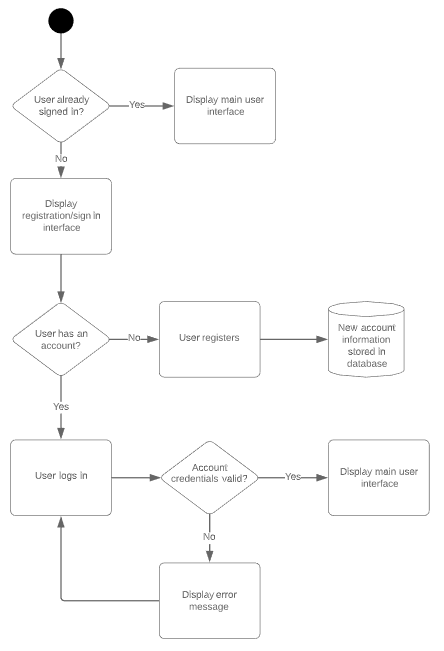
\includegraphics[width=120mm]{../figures/ActivityDiagramAuthentication}
            \caption{Activity Diagram: Authentication}
        \end{figure}

        \pagebreak

        \begin{figure}[!h]
            \center
            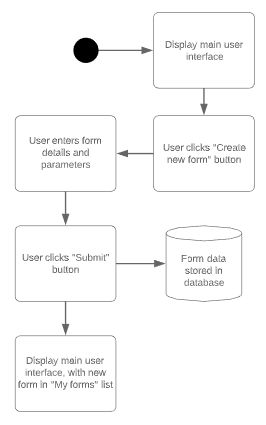
\includegraphics[width=120mm]{../figures/ActivityDiagramFormCreation}
            \caption{Activity Diagram: Form Creation}
        \end{figure}

        \pagebreak

        \begin{figure}[!h]
            \center
            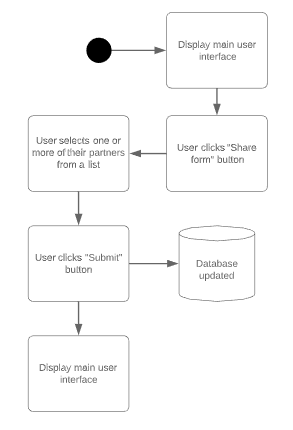
\includegraphics[width=120mm]{../figures/ActivityDiagramFormSharing}
            \caption{Activity Diagram: Form Sharing}
        \end{figure}

        \pagebreak

        \begin{figure}[!h]
            \center
            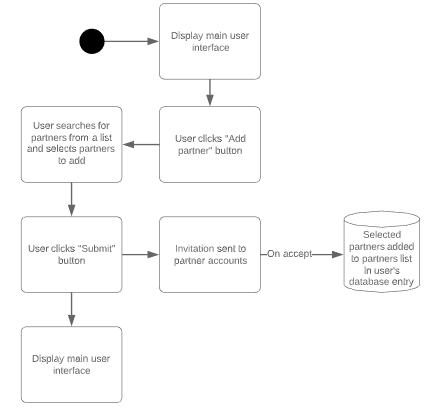
\includegraphics[width=120mm]{../figures/ActivityDiagramPartnerInvitation}
            \caption{Activity Diagram: Partner Invitation}
        \end{figure}

        \pagebreak

    \subsection{Model-View-Controller Diagram}

    \hfill\break

        \begin{figure}[!h]
            \center
            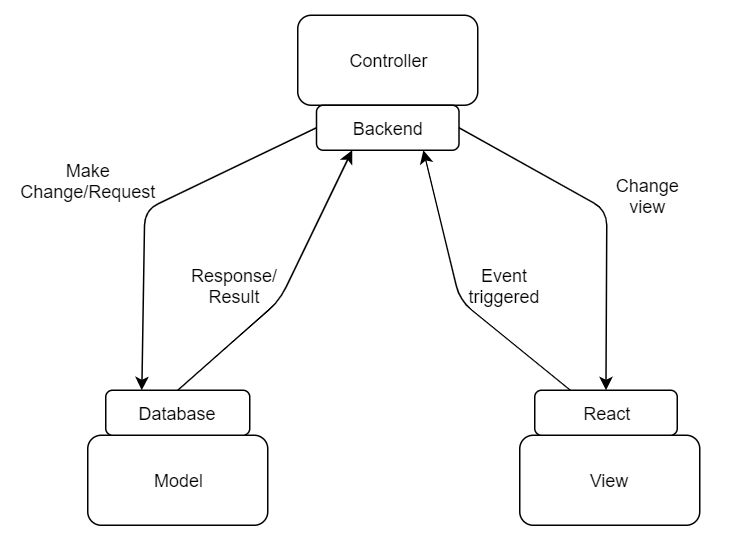
\includegraphics[width=155mm]{../figures/MVC}
            \caption{MVC Diagram}
        \end{figure}

\section{Validation}
    The testing and validation of the application will be done using Robot Framework. Robot Framework is a generic, open source, automation framework for acceptance testing \cite{Robot}, developed with Python. The framework has many libraries that extend its functionality, and one such library is Selenium, which will be used extensively to automatically drive the application\textquoteright s user interface. These tests will be written in conjunction with the application\textquoteright s features, and run alongside each check-in, as per the continuous integration methodology.